\documentclass[10pt,a4paper]{article}
%]{report}

\usepackage[a4paper, top=2cm, bottom=2.5cm, left=3cm, right=3cm]{geometry}
%\usepackage[
%    vmarginratio=2:2.5, %Verh�ltnis der oben/unten Seitenr�nder zur automatischen Berechnung
%    paper=a4paper,
%    lmargin=3cm, % mittlerer Rand
%    rmargin=3cm, % �u�erer Rand
%    marginparwidth=2.3cm, % Breite des Marginpars
%    includehead, % Kopfzeile in Berechnung einbeziehen
%    includemp % Marginpar in die Berechnung mit einbeziehen
%]{geometry}
%\setlength\marginparwidth{2.3cm} %Die wird sp�ter zum Rechnen gebraucht, wird aber durch die Angabe im geometry package nicht automatisch richtig gesetzt.


%============================================================
% Pakete
%============================================================

\usepackage[english, ngerman]{babel}    % mehrsprachiger Textsatz
% babel: letzte Sprache in Optionen zeigt die Sprache des Dokumentes
% und kann durch den Befehl \selectlanguage{} geaendert werden
% Passen Sie die Optionen des babel-Paketes nach Bedarf an!
\usepackage[utf8]{inputenc}       % Eingabekodierung Parameter latin1 darf ge�ndert werden
\usepackage[T1]{fontenc}                % Schriftenkodierung
\usepackage{graphicx}                       % zum Einbinden von Grafiken
\usepackage{lmodern}                        % Ersatz fuer Computer Modern-Schriften
                                                                % zum besseren Aussehen am Bildschirm
\usepackage{epstopdf}		% Grafiken einbinden
\usepackage{caption}		%Grafiken beschriften
%\usepackage{verbatimfiles}	% Ganze Dateien als Verbatim einbinden
% \usepackage{programs}	% Ganze Dateien als Verbatim einbinden
\usepackage{verbatim}		% Mehrzeilige Kommentare
\usepackage{multicol}		% Mehrere Spalten
\usepackage{hyphsubst}		% Silbentrennung
\usepackage{xcolor,soul}
\usepackage{float}				%Sachen an der richtigen Stelle ausgeben
\restylefloat{figure}				%Abbildungen an der richtigen Stelle ausgeben
\restylefloat{table}				%Tabellen an der richtigen Stelle ausgeben
\usepackage{array}				%f�r Tabellen
\newcolumntype{C}{>{$}c<{$}} 	%Tabellenspalten C mit mathematischem Inhalt
% \usepackage{subfigure}
\usepackage{ulem}				%doppelt unterstreichen
\usepackage{siunitx}
\usepackage{hyperref}
\usepackage{booktabs}
\usepackage{subcaption}

\usepackage{etex} %needs to be used to avoid 'no room error in pgfplots'
\usepackage{pgfplots}
\usepackage{tikz}
\usepackage{tikz-3dplot}
%\usepackage{tikzscale}
\usepgfplotslibrary{polar}
\usetikzlibrary[pgfplots.colormaps]
\pgfplotsset{compat=newest}
\pgfplotsset{plot coordinates/math parser=false}
\newlength\figureheight
\newlength\figurewidth
%\pgfplotsset{y tick label style={/pgf/number format/fixed}}
%\pgfplotsset{yticklabel style={text width=2.2em,align=right}}%,fixed zerofill, precision=1}}
%\pgfplotsset{every x tick/.append style={line width=1pt}}
%\pgfplotsset{every y tick/.append style={line width=1pt}}
%\pgfplotsset{every axis plot/.append style={line width=1.0pt}}
%\pgfplotscreateplotcyclelist{mycolorlist}{blue,red,green,brown,teal,orange,violet,cyan,green!70!black,magenta,gray}

\usepackage{tikzscale}
\usetikzlibrary{external}
\usetikzlibrary{fadings}
\usetikzlibrary{arrows}
\usetikzlibrary{calc}
\usetikzlibrary{plotmarks}
\usepgfplotslibrary{external}
\tikzset{external/force remake=false}
\tikzset{external/system call={pdflatex \tikzexternalcheckshellescape -halt-on-error -interaction=batchmode -jobname "\image" "\texsource"}}

\tikzexternalize

% define colors for source code list
\definecolor{colKeys}{rgb}{0,0,1}
\definecolor{colIdentifier}{rgb}{0,0,0}
\definecolor{colComments}{rgb}{0,1,0.3}
%\definecolor{colString}{rgb}{0,0.5,0}
\definecolor{dkgreen}{rgb}{0,0.6,0}
\definecolor{gray}{rgb}{0.5,0.5,0.5}
\definecolor{colString}{rgb}{0.63,0.13,0.94}

% Code-Listings print source code
\usepackage{listings}
\lstset{language=Python,		% choose the language of the code
	inputencoding=latin1,
	keywords={break,case,catch,continue,else,elseif,end,for,function,
	 global,if,otherwise,persistent,return,switch,try,while,ones,zeros},
   	float=hbp,
%  	 basicstyle=\ttfamily\small,				% the size of the fonts that are used for the code
   	identifierstyle=\color{colIdentifier},
   	keywordstyle=\color{blue},
   	commentstyle=\color{dkgreen},
  	stringstyle=\color{colString},
   	columns=flexible,
  	tabsize=2,								% sets default tabsize to 2 spaces
   	%frame=none; %single,
  	 numbers=left,						% where to put the line-numbers
  	 showspaces=false,                               % show spaces adding particular underscores
  	 numberstyle=\ttfamily\small\color{gray},
% numberstyle=\footnotesize,                      % the size of the fonts that are used for the line-numbers
  	 stepnumber=1,                                           % the step between two line-numbers. If it's 1 each line will be numbered
  	 numbersep=10pt,                                  % how far the line-numbers are from the code
  	 showspaces=false,
  	 showstringspaces=false,                         % underline spaces within strings
  	 breakautoindent=true,                        % sets if automatic breaks should only happen at whitespace
%       backgroundcolor=\color{white},          % choose the background color. You must add \usepackage{color}
%  	     showtabs=false,                                         % show tabs within strings adding particular underscores
%       frame=single,                                           % adds a frame around the code
%       captionpos=b,                                           % sets the caption-position to bottom
%        escapeinside={\%*}{*)                          % if you want to add a comment within your code
        breaklines=true}                                       % sets automatic line breaking

% Mathe-Pakete
\usepackage{amsfonts}
\usepackage{amsmath}
\usepackage{amsthm}		% Theorem-Umgebung, Beweise
\usepackage{amssymb}
\usepackage{cancel}
\usepackage{mathcomp}
\usepackage{nicefrac}

\usepackage{libertine}
\usepackage[libertine]{newtxmath}

%============================================================
% Titel, Autor, Datum
%============================================================
\title{Übung 5 \\Computational Physics III}
\author{Matthias Plock (552335) \and Paul Ledwon (561764)} %\\Otto Normalverbraucher (271828)}
\date{\today}

%============================================================
% Dokument
%============================================================
\begin{document}

% Titel erstellen
\maketitle
\tableofcontents

\pagenumbering{arabic}
\pagestyle{myheadings}                  % bzw. ist fancyhdr zu benutzten

\section{Conjugate-Gradient auf der GPU}

Die Funktionen aus den letzen Uebungen wurden so in das Grundgeruest von Uebung5.zip
eingefuegt, dass nun der Conjugate-Gradient-Algorithmus parallelisiert auf der GPU
ausgefuehrt werden kann. Fuer verschiedene Gittergroessen $N$ wurden die Laufzeiten
bei verschiedenen execution-configurations und 10 Durchlaufen ermittelt. Aus dem
Durchschnitt der Laufzeiten für ein festes $N$ wurde mit der schnellsten execution-configuration
der Speedup berechnet. Die Ergebnisse sind in Abb. 1 dargestellt. Mit steigender Gittergroesse
steigt auch der Speedup, auch wenn dieser erst ab $N=512$ den Wert $1$ uebersteigt.\\

\begin{figure}[H]
  \centering
  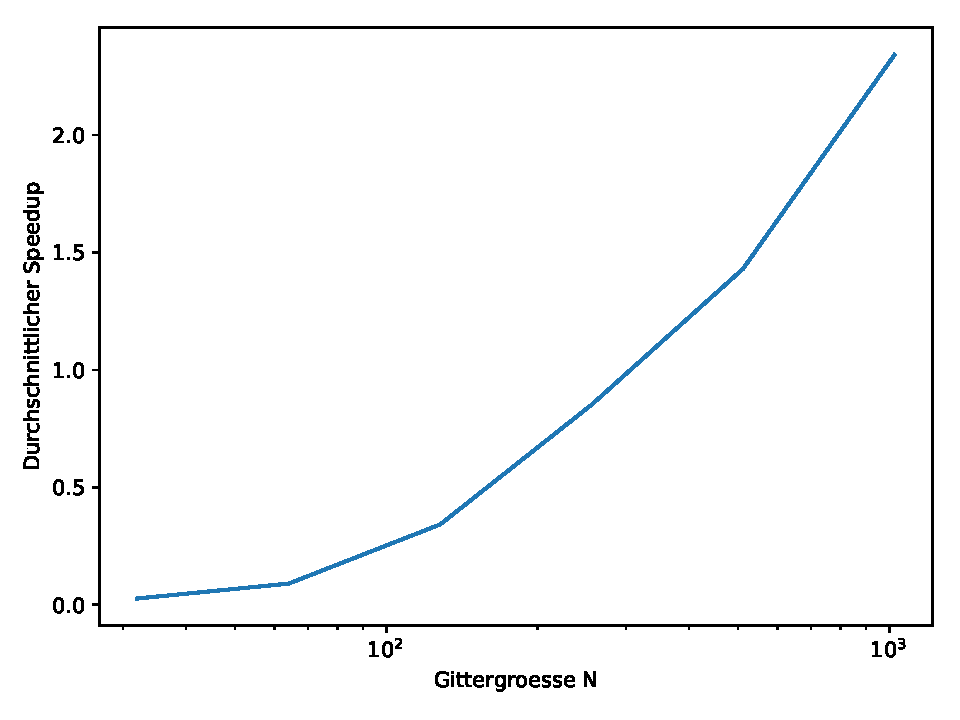
\includegraphics[width=\textwidth]{../figures/speedup.pdf}
  \caption{Bester durschnittlicher Speedup von verschiedenen execution-configurations}
\end{figure}


Es wird vermutet, dass die GPU-Implementierung nicht optimal ist, da bei der Benutzung von nvprof
auffiel, dass ein Grossteil der Laufzeit durch die Ausführung von den Unroll-Funktionen bei der Berechnungen
der Skalarprodukte verursacht wird. Um ein Skalarprodukt zu berechnen, wird unter anderem die Unroll-Funktion zweimal ausgefuehrt. Moeglicherweise
waere es effizienter, nur eine Unroll-Funktion auszufuehren und dann das vergleichsweise kleine Array seriell auf dem Host zu berechnen.




\section{Amdahlsches Gesetz}

Das Amdahlsche Gesetz besagt, dass fuer den Speedup $S_p(N) = \dfrac{T_s(N)}{T_p(N)}$
gilt

\begin{equation}
	S_p(N) \leq \frac{1}{f},
\end{equation}

wobei f der Anteil des Problems ist, der seriell ausgefuehrt werden muss.

\subsection{Beweis}

Wir teilen die Laufzeit der seriellen Loesung des Problems auf in

\begin{equation}
	T_s(N) = t_s + t^s_p = f \cdot T_s(N) + (1-f) \cdot T_s(N).
\end{equation}

Analog gilt dann fuer die Laufzeit des parallelen Problems

\begin{equation}
	T_p(N) = t_s + t^p_p = f \cdot T_s(N) + t^p_p.
\end{equation}

Hierbei ist $t_s$ die Laufzeit, die benoetigt wird um den seriellen Anteil des
Problems zu loesen. $t^s_p$ und $t^p_p$ sind die Laufzeiten, die das beste serielle bzw.
parallelisierte Programm zur Loesung des parallelisierbaren Anteils des Problems benoetigen.
Theoretisch kann $t^p_p$ auf die Dauer einer Operation reduziert werden, fuer den Fall,
dass man eine ausreichende Menge an Threads zur Verfuegung hat.

Setzt man (2) und (3) in die Definition des Speedups ein erhaelt man

\begin{align*}
	S_p(N) &= \dfrac{f \cdot T_s(N) + (1-f) \cdot T_s(N)}{f \cdot T_s(N) + t^p_p} \leq \dfrac{f \cdot T_s(N) + (1-f) \cdot T_s(N)}{f \cdot T_s(N)} \\
				 &= \dfrac{1 + \frac{1-f}{f}}{1} = \frac{f+1-f}{f} = \dfrac{1}{f}
\end{align*}


\end{document}
